\chapter{네트워크 이론}\label{cha:networktheory}

\section*{학습개요}

\section*{학습목표}
\begin{enumerate}
\item 네트워크를 분석하는 그래프 이론의 기초를 이해한다.
\item 네트워크 효과를 설명할 수 있다.
\item 양의 외부성과 양의 피드백을 설명할 수 있다.
\item 소비자의 지불 가능의사와 네트워크 효과의 관계를 이해할 수 있다.
\item 네트워크가 있는 시장에서 사용자 수의 초기 확보가 중요한 이유를 설명할 수 있다.
\end{enumerate}

\section*{주요 용어}
노드, 엣지,  네트워크 효과, 외부성, 양의 피드백, 규모의 경제, 지불가능의사, 임계 질량


\pagebreak


\section{그래프 이론}\label{sec:}
\begin{itemize}
\item 네트워크는 어디에서나 볼 수 있음 \citep{Jackson:2021aa}
	\begin{itemize}
	\item 가족, 결혼, 친구, 동료 등의 인간 관계
	\item 논문, 특허 인용 등의 연구 및 기술 확산
	\item 도로, 철로 등의 경로
	\item 질병의 전파, 대출의 연쇄 등
	\end{itemize}
\item 그래프 이론 (graph theory) $\rightarrow$ 네트워크를 수학적으로 표현
	\begin{itemize}
	\item 노드 (nodes): 종단점, 연결 대상, A, B 
	\item 에지 (edge) 또는 링크(link): 노드를 연결
		\begin{itemize}
		\item 방향이 있음(directed): A $\rightarrow$ B
			\begin{itemize}
			\item 일방통행 $\rightarrow$ 논문의 인용, 홈페이지 링크 등
			\end{itemize}
		\item 방향이 없음(undirected): A $\leftrightarrow$ B, 보통은 A --- B 로 표시
			\begin{itemize}
			\item 양방통행 $\rightarrow$ 계약, 동맹 등
			\end{itemize}
		\end{itemize}
	\end{itemize}
\item 기본 개념 \cite[Ch. 1]{Easley:2010aa}
	\begin{itemize}
	\item 경로 (path)
		\begin{itemize}
		\item 엣지로 연결된 노드 쌍의 순서
		\item[예)] SRI -- STAN -- UCLA -- SRI -- UTAH -- MIT 
		\end{itemize}
			\begin{figure}[htbp]
			\begin{center}
			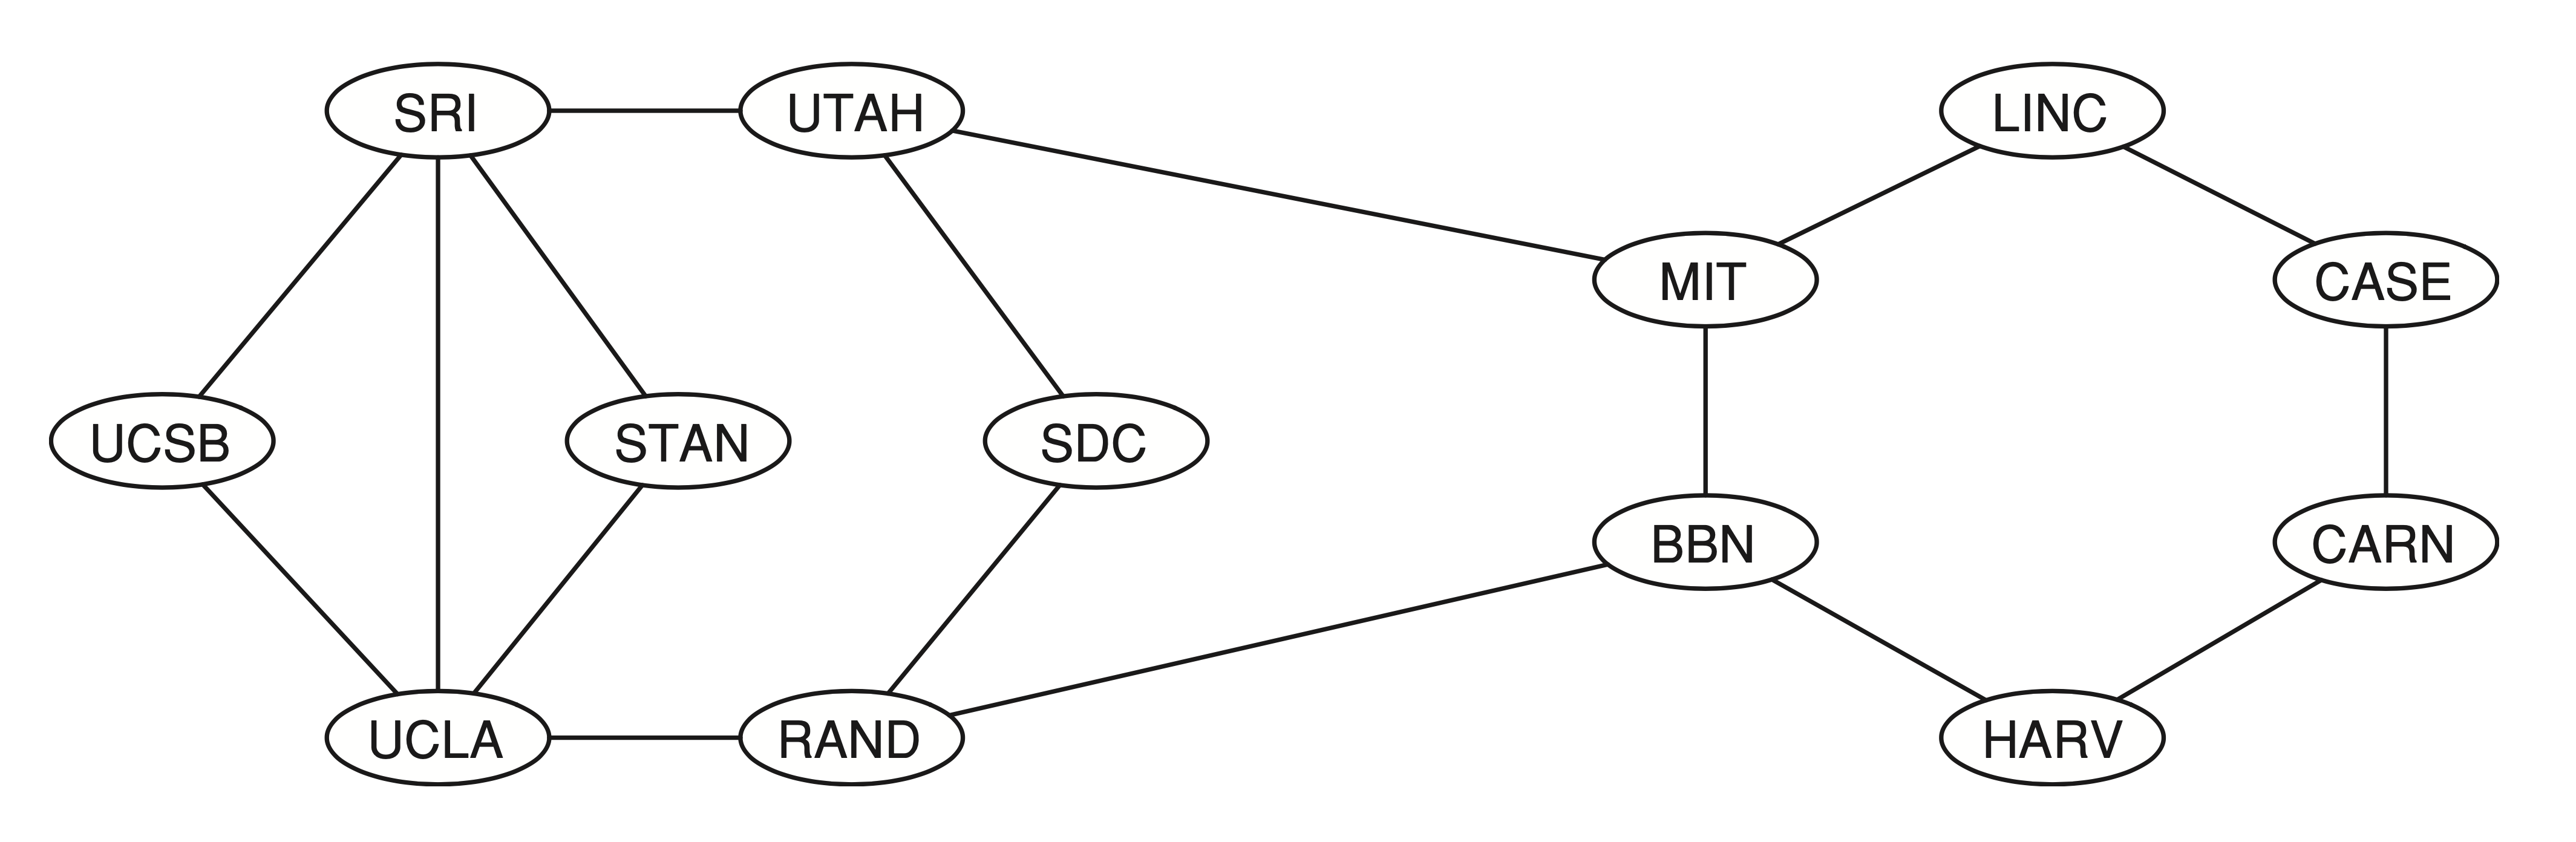
\includegraphics[scale=0.15]{Easley2010fig2_3.png}
			\caption{1970년 ARPANET}
			\label{fig:internetin1970}
			\end{center}
			\end{figure}
	\item 연결 (connected)
		\begin{itemize}
		\item 모든 노드 쌍에 경로가 있을 때 그래프가 연결되었다고 정의할 수 있음
		\item[예)] 그림 \ref{fig:internetin1970}
		\end{itemize}
	\item 컴포넌트 (component)
		\begin{itemize}
		\item 내부적으로 연결되어 있음
		\item 그래프의 다른 부분과 연결된 엣지가 없음
		\end{itemize}
	\item 경로의 길이 (length)
		\begin{itemize}
		\item 경로에 포함된 엣지의 수
		\item[예)] MIT -- BBN -- RAND -- UCLA $\rightarrow$ 3개
		\end{itemize}
	\item 두 노드의 거리 (distance)
		\begin{itemize}
		\item 두 노드의 가장 짧은 경로의 길이
		\item[예)] LINC -- SRI 의 거리: 3
		\item[활용)] 친구 -- 친구의 친구 -- 친구의 친구의 친구 -- $\cdots$
			\begin{itemize}
			\item ``작은 세계 현상 또는 분리의 여섯 단계(small-world phenomenon or six degrees of separation)"
			\end{itemize}
		\end{itemize}
	\end{itemize}		
\end{itemize}

\section{네트워크 효과}
\begin{itemize}
\item 네트워크가 경제 주체에 미치는 영향
	\begin{enumerate}
	\item 네트워크를 통해 정보를 전달
	\item 네트워크를 통해 이득을 전달 $\rightarrow$ 네트워크 효과
	\end{enumerate}
\item 네트워크 효과
	\begin{itemize}
	\item 어떤 재화나 서비스의 사용자 수가 늘어날 수록 그 가치가 더 높아짐\footnote{네트워크의 규모를 측정하면, 네트워크의 가치를 어림짐작할 수 있음. 네트워크의 규모를 측정하는 방법으로는 $n$개의 노드가 있을 때, 연결 방법에 따라 $n$ (사르노프의 법칙, Sarnoff's Law), $2^{n}$ (리드의 법칙, Reed's law), $n^{2}$ (멧칼프의 법칙, Metclafe's Law) 등으로 측정할 수 있다.}
	\end{itemize}	
\item $\rightarrow$ 네트워크의 양의 외부성
	\begin{itemize}
	\item 외부성
		\begin{itemize}
		\item 어떤 경제 행위가 제 3자에게 누출 편익(spillover benefit) 또는 누출 비용(spillover cost)을 주는 것
		\item 양의 외부성(또는 외부경제)
			\begin{itemize}
			\item 타인에게 누출 편익을 줄 때
			\item[예)] 어떤 집 주인이 집의 색을 바꾸고 정원을 꾸밈 $\rightarrow$ 이웃은 그로부터 즐거움을 느낄 수 있음 $\rightarrow$ 하지만 주인은 이웃의 그런 이득에 대해 이웃으로부터 대가를 받지 않음
			\end{itemize}
		\item 음의 외부성(또는 외부불경제)
			\begin{itemize}
			\item 타인에게 누출 비용을 부과할 때
			\item[예)] 운전자는 자신의 목적에 따라 차량을 운전 $\rightarrow$ 도로 용량을 넘는 차량이 몰리면 교통 체증이 시작 $\rightarrow$ 통행 시간의 증가(비용 발생), 하지만 각 운전자는 서로에게 비용을 지불하지 않음
			\end{itemize}
		\end{itemize}
	\item 네트워크의 양의 외부성
		\begin{itemize}
		\item 네트워크에 연결되어 있는 것의 가치가 네트워크의 크기와 함께 증가하기 때문		
		\item[예)] 다른 사람이 아래아 한글을 쓸 때는 아래아 한글을, MS 워드를 쓰고 있다면 MS 워드를 쓰는 것이 유리
		\end{itemize}
	\end{itemize}
\item 직접 대 간접
	\begin{itemize}
	\item 직접: 거리가 짧은 노드로 부터 얻는 효과
		\begin{itemize}
		\item 친구의 정보
		\end{itemize}
	\item 간접:  거리가 먼 노드로 부터 얻는 효과
		\begin{itemize}
		\item[예)] 게임 사용자 수의 증가 $\rightarrow$ 게임 개발사 유인, 운영 체제 사용자 증가 $\rightarrow$ 응용 프로그램 개발 유인
		\end{itemize}
	\end{itemize}
\item 네트워크에서 발생하는 양의 외부성은 양의 피드백을 가져옴	
	\begin{itemize}
	\item 양의 피드백
		\begin{itemize}
		\item 어떤 요인이 결과를 만들고, 이 결과가 다시 바로 그 요인을 더 강화시킴
		\item 양의 피드백이 있으면 강한 것은 더욱 강해지고, 약한 것은 더욱 약해짐
			\begin{itemize}
			\item 성장과는 다른 의미
			\item 양의 피드백은 하나의 방향으로 강화된다는 의미
			\item $\rightarrow$ 양의 피드백은 성장을 강화하기도 하지만 실패를 강화하기도 함
			\end{itemize}
		\end{itemize}
	\end{itemize}
\end{itemize}

\section{네트워크 효과의 경제적 의미}
\begin{itemize}
\item 수요에서 규모의 경제(Economies of Scale)
	\begin{itemize}
	\item 보통은 공급에서 규모의 경제: 생산량 증가함에 따라 평균 생산 비용 감소
	\item 수요에서 규모의 경제: 사용자 수의 증가에 따라 소비자가 부담할 비용의 감소
	\item[예)] 수강생이 많을 수록, 문제 해결을 위해 물어볼 수 있는 사람이 많아짐 $\rightarrow$ 질문/탐색의 비용이 낮아짐
	\end{itemize}
\item 소비자의 지불가능의사
	\begin{itemize}
	\item 재화나 서비스로부터 얻을 것으로 기대하는 효용에 따라 변화
	\item 네트워크 효과 $\rightarrow$ 소비자의 기대 효용을 높임 $\rightarrow$ 지불가능의사를 높임
		\begin{itemize}
		\item 어떤 소비자 $x$의 지불가능의사 $WTP_{x}$
		\item 어떤 재화나 서비스의 사용자 수가 $z$이고, 이로 인해 소비자가 얻는 이득을 $f(z)$라 하면
			\begin{itemize}
			\item 단, $0<z<1$ 이고, $f(\cdot)$는 $z$에 대해 증가 함수
			\item 즉, $z$가 증가함에 따라 그 값이 커지는 함수
			\end{itemize}
		\item 네트워크 효과가 있을 때의 지불가능의사는 $f(z)WTP_{x}$
		\end{itemize}
	\item 이 재화나 서비스의 가격이 $p$라면
		\begin{itemize}
		\item 소비자 $x$는 $f(z)WTP_{x} \geq p$ 일 때만 소비
		\end{itemize}
	\item 즉, 소비자 $x$가 예상하는 다른 소비자의 수 $z$ 가 중요
		\begin{itemize}
		\item 예상하는 다른 소비자 $z = 0$ 이라면 $\rightarrow$ 소비하지 않을 것
		\item 예상하는 소비자의 수가 충분하지 않다면 ($0< z < z^{'}$)
			\begin{itemize}
			\item $\rightarrow$ 다른 소비자도 그런 예상을 하고 있다면, 이 재화나 서비스에 대한 수요가 계속 감소 
			\item $\rightarrow$ 지불가능의사는 0으로 수렴
			\end{itemize}
		\item 예상하는 소비자의 수가 충분하다면 ($ z^{'} < z <  z^{''}$)
			\begin{itemize}
			\item $\rightarrow$ 다른 소비자도 그런 예상을 하고 있다면, 소비자 수가 계속 증가
			\end{itemize}
		\item 예상하는 소비자의 수가 너무 많다면 ($z^{''} < z < 1$)
			\begin{itemize}
			\item $\rightarrow$ 지불가능의사에 비해 가격이 너무 높으므로 소비가 감소 
			\item $\rightarrow$ 하지만 예상 소비자의 수가 많은 수준 근처에서 머물 것
			\end{itemize}
		\end{itemize}
	\end{itemize}
	
	\begin{figure}[htbp]
	\begin{center}
	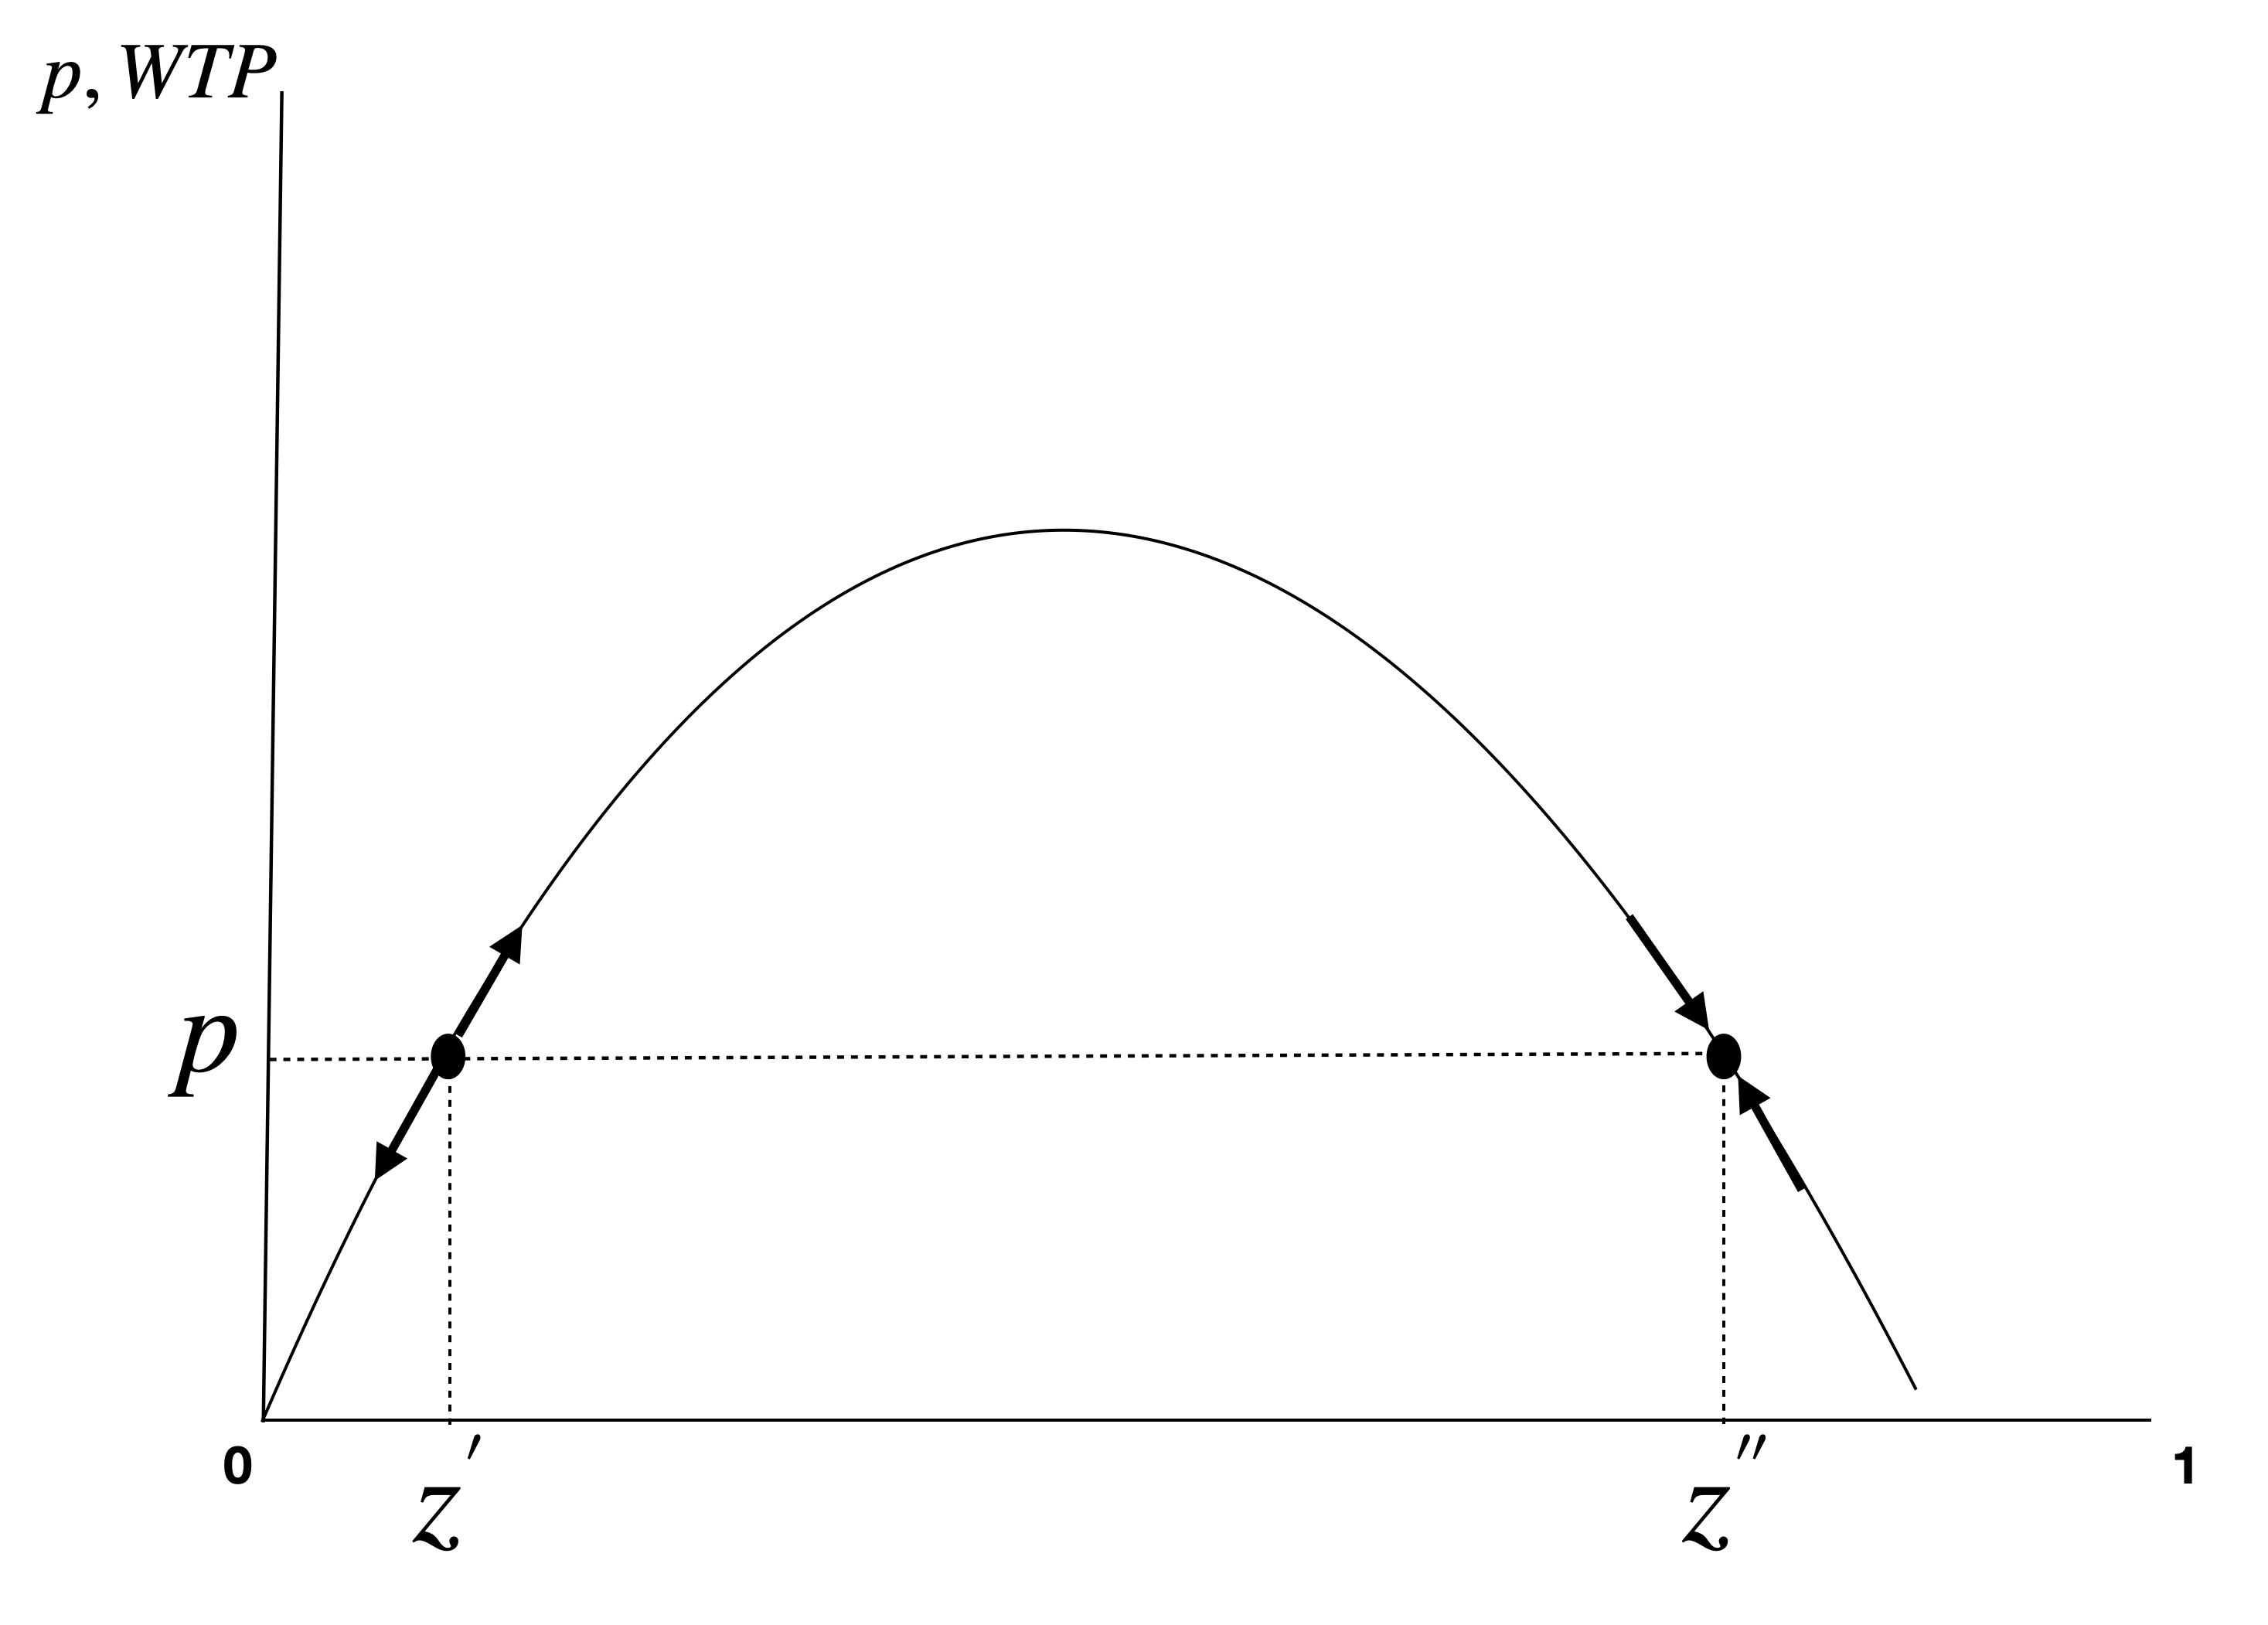
\includegraphics[scale=0.2]{criticalmass.png}
	\caption{네트워크 효과가 있는 시장에서의 균형}
	\label{fig:criticalmass}
	\end{center}
	\end{figure}

	
	
\item 임계 질량(critical mass)
	\begin{itemize}
	\item 우리는 스스로 지속 가능한(self-sustaining) 규모로 정의: ``알아서 잘 굴러가는"  $\rightarrow$ 양면 모두에서 필요할 수 있음
		\begin{itemize}
		\item 임계 질량은 원래 핵분열성 물질이 연쇄 반응을 일으킬 수 있는 최소의 질량을 의미 
		\item 핵분열성 물질의 핵에 중성자가 충돌하면 핵분열이 일어남 $\rightarrow$ 다시 중성자를 방출 $\rightarrow$ 이 중성자가 다시 근처의 핵에 충돌 $\rightarrow$ 연쇄 반응 
		\item 만약 충분한 야의 핵분열성 물질이 있지 않다면, 방출된 중성자가 근처의 핵에 충돌하지 않고 연쇄 반응이 일어나지 않을 수 있음. 플루토늄 239의 임계 질량은 약 11kg(24.2파운드)
		\end{itemize}
	\end{itemize}	
\item $\rightarrow$ 사용자 수의 초기 확보와 유지가 중요: \ref{cha:ecommerce}--\ref{cha:chikenandeggproblem} 장의 주제
	\begin{itemize}
	\item 지금까지의 논의만 생각해보면
		\begin{itemize}
		\item $p$가 낮은 수준이면, 즉 가격을 낮추면,
		\item $z^{'}$를 낮은 수준으로 $z^{''}$를 높은 수준으로 유지할 수 있음
		\item $\rightarrow$ 하지만, 기업은 손실을 입을 수 있음
		\item $\rightarrow$ 그러나, 시소 원칙과 같이 생각해볼 것
		\item $\rightarrow$ 또, 사용자 수의 증가로 인해 사업 영역의 확대도 가능
		\end{itemize}
	\item 페이스북(Facebook)
		\begin{itemize}
		\item 하버드 대학교와 그외 아이비리그 대학생의 회원 가입
		\item $\rightarrow$ 회원 대상의 증가
		\item $\rightarrow$ 게임(Farmville)과 어플리케이션
		\item $\rightarrow$ 타겟 광고
		\end{itemize}
	\item 에어비앤비(Airbnb) 등 다른 기업 사례
		\begin{itemize}
		\item \url{https://www.slideshare.net/a16z/network-effects-59206938} (영문)
		\end{itemize}	
	\end{itemize}
\item 네트워크 효과가 강한 산업
	\begin{itemize}
	\item 높은 진입 장벽으로 작동 
	\end{itemize}
\end{itemize}

\pagebreak

\section*{정리하기}
\begin{enumerate}
\item 네트워크는 노드와 링크로 연결되어 있는 구조이고, 주로 양의 외부성을 일으킨다. 
\item 네트워크에서 양의 외부성은 양의 피드백을 가져온다.
\item 양의 외부성은 어떤 경제 행위가 제3자에게 누출 편익을 주는 것이다.
\item 양의 피드백은 어떤 요인이 결과를 만들고 이 결과가 다시 그 요인을 더 강화시키는 것으로, 양의 피드백이 있으면, 어느 하나의 방향이 강화되는 효과가 나타난다.
\item 네트워크 효과는 소비자의 지불가능의사를 높이고, 소비자의 지불 가능의사가 소비자의 수에 따라 역 U자의 형태를 갖는다고 할 때, 예상하는 전체 소비자의 수가 적은 상태는 기대 효용이 주어진 가격보다 낮아지게 되어 결국 소비를 하지않게 된다. 그리고 양의 피드백으로 이 방향은 더욱 강화된다. 따라서 적은 수의 소비자는 안정적인 균형이 아니다.
\item 하지만, 예상하는 전체 소비자의 수가 많은 상태에서는 그 소비자 수가 더 늘어 소비기대 효용이 주어진 가격보다 낮아지더라도, 결국 많은 수준의 예상 소비자 수준으로 복귀한다. 따라서 많은 수의 소비자는 안정적인 균형이다.
\item 이는 네트워크 효과가 있는 시장에서 일정 수의 소비자 수를 확보하면 안정적으로 사업을 운영할 수 있음을 의미하고 이를 임계 질량이라고 할 수 있다.
\item 따라서 네트워크 효과가 있는 시장에서는 사용자 수의 초기 확보와 유지가 중요하다. 가장 간단한 전략은 가격을 낮춰 안정적인 소비자 수가 될 수 있는 수준을 낮추는 것이다.
\item 가격을 낮추더라도 양면 시장에서의 시소 원칙을 사용하면 플랫폼은 손해를 보지 않을 수 있고, 다른 한편 사용자 수를 늘리게 되면 다른 사업으로의 확장이 가능해진다.
\item 그러나 사용자 수를 초기에 확보하는 것이 쉬운 일은 아니므로 네트워크 효과가 강한 시장에 신규 기업이 진입하기 어려운 진입 장벽이 될 수 있다.
\end{enumerate}